\begin{figure*}[!h]
\centering
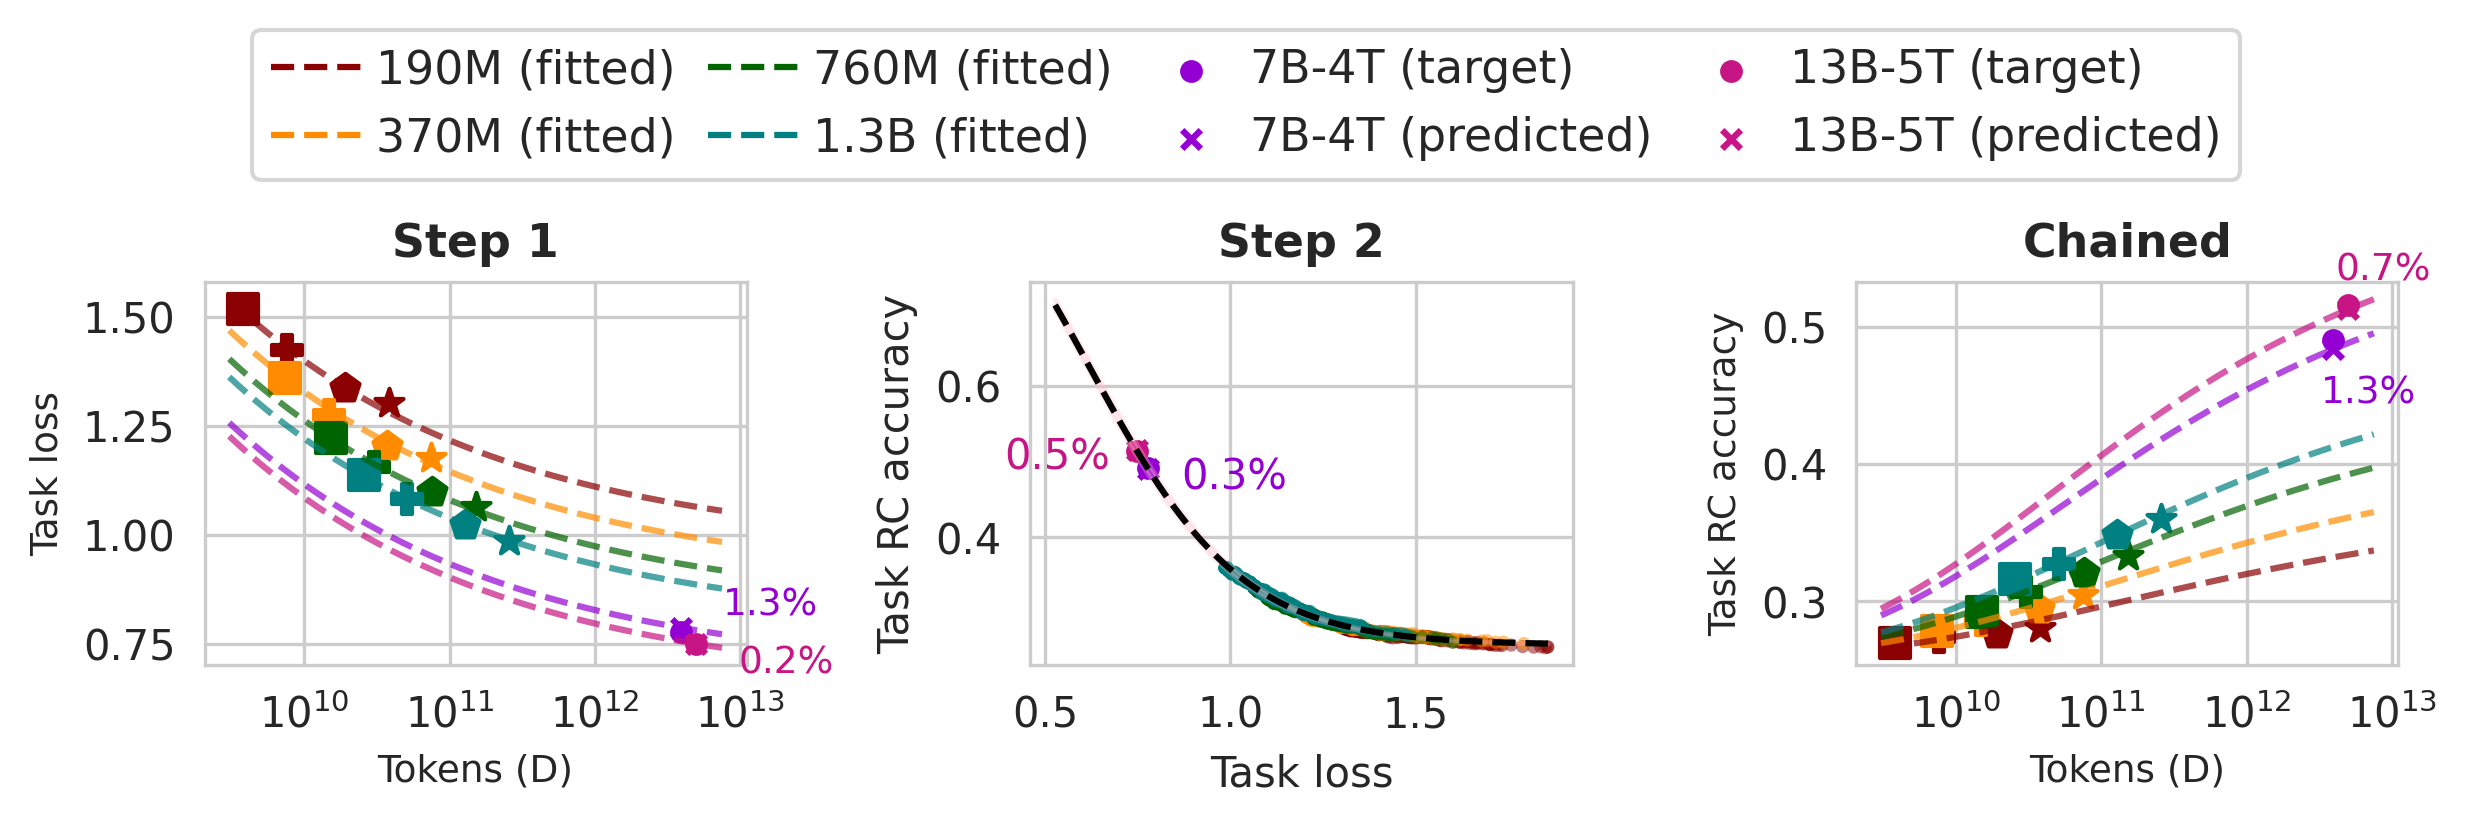
\includegraphics[width=0.9\linewidth]{images/figure1.png}
\vspace{-12pt}
\caption{
    Predicting MMLU accuracy with our method.
    We use model size $N$ and data size $D$ to predict a ``task loss'' on MMLU (step 1), and then use this task loss to predict task accuracy in ranked classification format (step 2).
    The chained plot shows end-to-end prediction from ($N$, $D$) to task accuracy.
    The functions in step 1 and 2 are fitted on data points collected from \textit{ladder} models (markers colored in red, orange, green and cyan); 7B-4T and 13B-5T are the target models for which we make predictions.
    We report relative prediction error in the plot next to each target model point.
    %\pw{fonts in the subplots should be consistent (e.g., step 2 has larger font). These plots would look better if they were taller---I wonder if you could move the legend to the right, and then squeeze the plots horizontally but make them taller?}
}
\label{fig:figure1}
\vspace{-8pt}
\end{figure*}